% ************************** Thesis Chapter3 **********************************
\chapter{ระเบียบวิธีวิจัย}
ในการทําโครงการวิจัยเครื่องมือกำกับคุณลักษณะด้วยปัญญาประดิษฐ์ จะมีการทำงานหลากหลายส่วนมาทำงานร่วมกัน 
ซึ่งต้องมีระเบียบวิธีวิจัยอธิบายถึงขั้นตอนการดำเนินงานตั้งแต่เริ่มศึกษาข้อมูลจนไปถึงสิ้นสุดกระบวนการวิจัย
\section{ความต้องการของระบบ}
\subsection{ความต้องการเชิงการใช้งาน (functional requirements)}
\begin{enumerate}
	\setlength\itemsep{-0.25em}
    \item เครื่องมือกำกับคุณลักษณะด้วยปัญญาประดิษฐ์ต้องสามารถตัดวิดิโอช่วงเวลาที่ไม่มีมนุษย์อยู่ออกได้อัตโนมัติโดยใช้ปัญญาประดิษฐ์ 
	\item เครื่องมือกำกับคุณลักษณะด้วยปัญญาประดิษฐ์สามารถระบุตำแหน่งมนุษย์แต่ละคนในวิดีโอและจำแนกการกระทำของมนุษย์ในวิดีโอได้ 
	โดยการกระทำที่กำหนดจะประกอบไปด้วย ยืน นั่ง นอน เล่นโทรศัพท์ เดิน กินข้าว พูดคุย
	\item ชุดข้อมูลที่ได้จากเครื่องมือกำกับคุณลักษณะด้วยปัญญาประดิษฐ์ต้องสามารถนำไปใช้ในการพัฒนาโมเดลปัญญาประดิษฐ์ต่อได้ 
	\item สร้างระบบต้นแบบของเครื่องมือกำกับคุณลักษณะด้วยปัญญาประดิษฐ์ที่มนุษย์สามารถทำงานร่วมกับปัญญาประดิษฐ์ได้
	\item ระบบวิเคราะห์การกระทำมนุษย์ต้องสามารถนำวิดีโอมาวิเคราะห์ข้อมูลการกระทำและตำแหน่งของมนุษย์แต่ละคน แล้วนำข้อมูลเหล่านั้นไปสร้างรายงานที่มีคำกำกับออกมาได้ โดยรายละเอียดรายงานจะมีดังนี้
	\begin{enumerate}
		\item เวลา (time stamp)
		\item การกระทำ ซึ่งประกอบไปด้วย ยืน นั่ง เดิน เล่นโทรศัพท์ กินข้าว นอน
		\item ตำแหน่ง โดยจะบอกในลักษณะของกรอบสี่เหลี่ยมครอบพื้นที่ที่มนุษย์คนนั้นๆอยู่
	\end{enumerate}
\end{enumerate}
\subsection{ความต้องการเชิงวิศวกรรม (non-functional requirements)}
\begin{enumerate}
	\setlength\itemsep{-0.25em}
	\item สร้างเครื่องมือกำกับคุณลักษณะด้วยปัญญาประดิษฐ์โดยใช้ภาษาไพธอน
	\item ความละเอียดอย่างต่ำของวิดีโอต้องมากกว่า 640 x 480 (กว้าง x สูง) 
	\item วิดีโอจะต้องมีอัตราเฟรมต่อวินาทีอย่างต่ำ 10 เฟรมต่อวินาที
\end{enumerate}
\clearpage

\section{ภาพรวมระบบของเครื่องมือกำกับคุณลักษณะด้วยปัญญาประดิษฐ์}
\begin{figure}[!ht]
    \centering
    \includegraphics[width=0.6\textwidth, height=1.0\textwidth]{chapter3/images/Overview/HowItWorks.png}
    \caption{ภาพรวมระบบของเครื่องมือกำกับคุณลักษณะด้วยปัญญาประดิษฐ์}
    \label{fig:labeling_overview}
\end{figure}
\clearpage

\section{หน้าที่ความรับผิดชอบ} 
\paragraph*{ปฐมพงศ์ สินธุ์งาม}
สร้างและทดสอบโมเดลปัญญาประดิษฐ์สำหรับจดจำการกระทำมนุษย์ I3D รวมถึงออกแบบและสร้างระบบ Tracker
\paragraph*{ศุภกร เบญจวิกรัย}
รวมฟังก์ชั่นและระบบต่างๆของเครื่องมือ รวมถึงออกแบบและสร้างระบบ Select และ Detect
\paragraph*{อุกฤษฎ์ เลิศวรรณาการ}
สร้างและทดสอบโมเดลปัญญาประดิษฐ์สำหรับจดจำการกระทำมนุษย์ Resnet-50 รวมถึงออกแบบและสร้างระบบ Person ReID 

\vspace{6mm}
\section{เครื่องมือที่ใช้ในงานวิจัย}
ในหัวข้อนี้จะกล่าวถึงซอฟต์แวร์ ภาษา และ program library ที่ใช้ในการพัฒนาระบบ รวมถึงข้อมูลจำเพาะของคอมพิวเตอร์ที่ใช้ในการพัฒนาระบบ
\subsection*{Pycharm community 2017.1.2} 
เป็นโปรแกรมไว้ใช้สำหรับเขียนและแก้ไขโค้ดซึ่งข้อดีของโปรแกรมนี้ คือ มีคุณสมบัติต่างๆที่สามารถอำนวยความสะดวกในการเขียนโปรแกรมได้ เช่น 
syntax highlighting, auto-completion ฯลฯ และสามารถประมวลผลโปรแกรมทดสอบแอปพลิเคชันได้

\subsection*{Jupyter 2017.1.2} เป็นโปรแกรมสำหรับเขียนโปรแกรมที่เหมาะสำหรับใช้ในการทดสอบโปรแกรมแต่ละส่วนได้ ซึ่งมีข้อดีคือ 
หากมีการแก้ไขโปรแกรมเพียงแค่บางส่วน ก็สามารถประมวลผลเฉพาะส่วนที่ต้องการได้มักจะใช้ในการสร้างโมเดลปัญญาประดิษฐ์

\subsection*{Qt Creator 4.9.2 (community)}
เป็นเครื่องมือสำหรับออกแบบหน้าต่างแอปพลิเคชันของ library PyQt ซึ่งมีข้อดีคือ เรียกใช้ง่ายมีวิดเจ็ต (widget) ที่สามารถใช้ได้หลากหลายเหมาะสำหรับการออกแบบ

\clearpage
\section{ภาษาที่ใช้ในการพัฒนาระบบ} 
	ใช้ภาษาไพธอนในการพัฒนาเป็นหลัก เพราะเป็นภาษาที่ปัจจุบันมีการใช้กันอย่างแพร่ มีเครื่องมือและ library ที่อำนวยความสะดวกในการพัฒนามากมาย 
	ทั้งยังเป็นภาษาที่สามารถเข้าใจได้ง่าย โดยในการทำวิจัยครั้งนี้ได้เลือก python 3.6.8 มาใช้ในการพัฒนา 
	เนื่องจากเป็นรุ่นที่รองรับการทำงานของ library Tensorflow 1.12 และ CUDA 9
\vspace{3mm}
\section{Program library ที่ใช้ในการพัฒนาระบบและแอปพลิเคชัน} 
\begin{tabular}{|c|c|c|}
		\hline
		{Library}&{Version}&{Description}\\
		\hline
		numpy	 			& 1.16.4		& library ใช้สำหรับการคำนวณและ array			\\
		pandas				& 0.24.2		& library ใช้สำหรับการจัดการข้อมูลที่อยู่ในรูปแบบของ excel				\\
		opencv			 	& 4.1.0.25		& library ใช้สำหรับการจัดการข้อมูลที่เป็นรูปภาพและวิดีโอ		\\
		pillow				& 6.0.0			& library ใช้สำหรับการจัดการข้อมูลที่เป็นรูปภาพ			\\
		torchsummary		& 1.5.1			& library ใช้สำหรับการวิเคราะห์โครงสร้างของโมเดล 							\\
		pytorch		 		& 1.10.0		& library ใช้สำหรับการสร้างปัญญาประดิษฐ์							\\
		torchvision			& 0.3.0	 		& library ใช้สำหรับการสร้างปัญญาประดิษฐ์							\\
		scikit-learn		& 0.21.2		& library ใช้สำหรับการสร้างปัญญาประดิษฐ์							\\
		scipy				& 1.3.0			& library ใช้สำหรับการสร้างปัญญาประดิษฐ์							\\
		sklearn				& 0.0			& library ใช้สำหรับการสร้างปัญญาประดิษฐ์							\\
		pickleshare			& 0.7.5			& library ใช้สำหรับการทำถอดรหัส (encoding) โมเดลปัญญาประดิษฐ์			\\
		tqdm				& 4.32.1		& library ใช้สำหรับจัดการการทำงานซ้ำ (loop)					\\
		pyqt5				& 5.9.2			& library ใช้สำหรับการทำแอปพลิเคชัน					\\
		\hline
\end{tabular}

\vspace{3mm}
\section{แผนการดำเนินงาน}
โดยจากที่กล่าวไปตอนต้นในบทนำการดำเนินงานและการออกแบบการสร้างเครื่องมือกำกับคุณลักษณะด้วยปัญญาประดิษฐ์
และระบบวิเคราะห์การกระทำของมนุษย์ในวิดีโอ มีแผนการทำงานซึ่งถูกแบ่งออกเป็นสามขั้นตอนดังนี้
\begin{enumerate}
	\setlength\itemsep{-0.25em}
	\item ศึกษาหาความเป็นไปได้ รวมถึงเทคโนโลยีในปัจจุบันที่เกี่ยวกับการสร้างแอปพลิเคชัน และการจำแนกการกระทำของมนุษย์ด้วยปัญญาประดิษฐ์ 
	เพื่อศึกษาและทำความเข้าใจ ข้อดี-ข้อเสีย ของเทคนิคหรือกระบวนการต่างๆ เพื่อนำมาประยุกต์ใช้กับงานวิจัยนี้
	\item ออกแบบและสร้างแอปพลิเคชันที่ใช้ในการสร้างชุดข้อมูลสำหรับการเทรนโมเดลจากวิดีโอ
	\item ออกแบบและสร้างระบบวิเคราะห์การกระทำของมนุษย์ได้โดยมีข้อกำหนดตามที่กล่าวไว้ในบทนำ
\end{enumerate}
\clearpage

ในการศึกษาเกี่ยวกับการออกแบบและการสร้างแอปพลิเคชันที่ใช้ในการสร้างชุดข้อมูลสำหรับการสร้างโมเดลจากวิดีโอ 
สิ่งที่ต้องให้ความสนใจคือฟังก์ชันการทำงาน การออกแบบและการจัดวางองค์ประกอบต่างๆในหน้าต่างแอปพลิเคชัน
และความสะดวกในการใช้งาน จากนั้นจึงเริ่มศึกษาเกี่ยวกับ library ที่ใช้ในการสร้างแอพพลิเคชั่น
ส่วนการศึกษาเกี่ยวกับการสร้างระบบวิเคราะห์การกระทำมนุษย์ จะมุ่งความสนใจไปที่ชุดข้อมูลสำหรับการวิเคราะห์วิดีโอ
โมเดลสำหรับการวิเคราะห์วิดีโอ เทคนิคในการสร้างโมเดล เทคโนโลยีในการทำระบบวิเคราะห์วิดีโอ
เพื่อใช้ในการออกแบบและสร้างระบบวิเคราะห์การกระทำของมนุษย์ในวิดีโอให้มีประสิทธิภาพ
ในบทนี้ก็จะกล่าวถึงกระบวนการออกแบบและการดำเนินการตามแผนที่วางเอาไว้
\section{การออกแบบหน้าต่างแอปพลิเคชันของเครื่องมือกำกับคุณลักษณะด้วยปัญญาประดิษฐ์}
การออกแบบเครื่องมือสำหรับกำกับข้อมูลด้วยปัญญาประดิษฐ์้น ผู้วิจัยได้เลือกใช้ library PyQt และภาษาไพธอนในการพัฒนา
เนื่องจาก PyQt นั้นเป็น library ที่มีผู้พัฒนาใช้กันอย่างแพร่หลาย จึงสะดวกในการศึกษา หาข้อมูลในการสร้างหรือแก้ไข
อีกทั้งยังเป็น library ที่สามารถพัฒนาด้วยภาษาไพธอนได้ และใช้งานง่าย สามารถปรับปรุงแก้ไขได้สะดวก

\subsection{เครื่องมือสำหรับกำกับข้อมูลด้วยปัญญาประดิษฐ์}
แอพพลิเคชั่นแบ่งการทำงานออกเป็นสี่ส่วนประกอบด้วยกระบวนการ Select, Detect, Track และ Label
เพื่อช่วยแบ่งเบาภาระของผู้พัฒนาในการสร้างชุดข้อมูลสำหรับสร้างโมเดลจากข้อมูลประเภทวิดีโอ โดยกระบวนการ Select
จะต้องสามารถตัดวิดีโอส่วนที่ไม่มีมนุษย์อยู่ออกจากวิดีโอได้ จากนั้นกระบวนการ Detect จะต้องหาตำแหน่งของมนุษย์ภายในวิดีโอได้
แล้วใช้กระบวนการ Track ทำนายตำแหน่งต่อไปของมนุษย์ข้อมูลตำแหน่งของมนุษย์ที่ได้จากกระบวนการ Detect
และกระบวนการ Label นั้นต้องสามารถทำนายการกระทำพื้นฐานของมนุษย์ได้ เช่น ยืน เดิน นั่ง กินข้าว หรือ นอน เป็นต้น 
โดยทุกส่วนการทำงานมนุษย์ต้องสามารถทำงานร่วมกับปัญญาประดิษฐ์ได้
ดังรูปที่ \ref{fig:labeling_overview}

\begin{figure}[!ht]
    \centering
    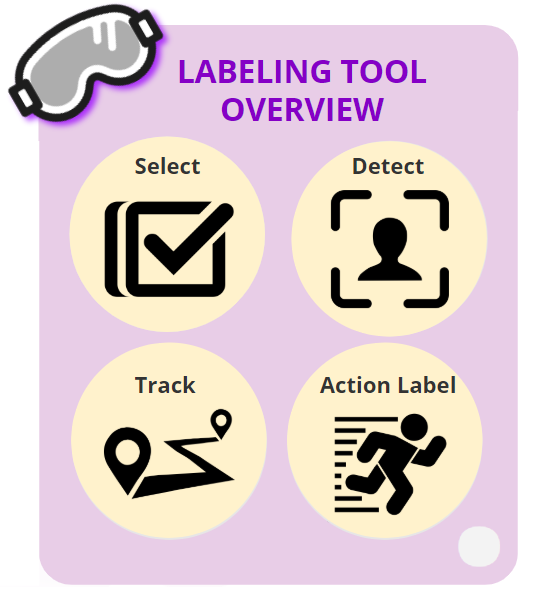
\includegraphics[width=0.5\textwidth]{chapter3/images/3_6/labelingToolOverview.png}
    \caption{กระบวนการหลักของเครื่องมือสำหรับกำกับข้อมูลด้วยปัญญาประดิษฐ์}
    \label{fig:labeling_overview}
\end{figure}
\clearpage

\subsection*{โดยแต่ละกระบวนการจะมีรายละเอียดดังนี้}
\subsubsection{Select}
กระบวนการ Select จะต้องสามารถรับวิดีโอเข้ามา แล้วตัดวิดีโอในช่วงที่ไม่มนุษย์อยู่ในเฟรมออกได้อัตโนมัติด้วยปัญญาประดิษฐ์
แต่เนื่องจากการประมวลผลทุกเฟรมในวิดีโอนั้นจะทำให้เสียเวลามากเกินไป จึงใช้วิธีการเลือกตัวอย่างเฟรมด้วยอัตราคงที่ (สามารถกำหนดได้)
ซึ่งเรียกว่าเฟรมเหล่านี้ว่า คีย์เฟรม จากนั้นใช้ปัญญาประดิษฐ์ประมวลผลคีย์เฟรมที่เหล่านั้น 
เพื่อลดระยะเวลาในการประมวลผลลง และมนุษย์จะต้องสามารถแก้ไขข้อผิดพลาดของปัญญาประดิษฐ์ได้ 
เพื่อเพิ่มคุณภาพของชุดข้อมูล จึงออกแบบหน้าต่างได้ดังรูปที่ \ref{fig:SelectDraft}

\begin{figure}[!ht]
    \centering
    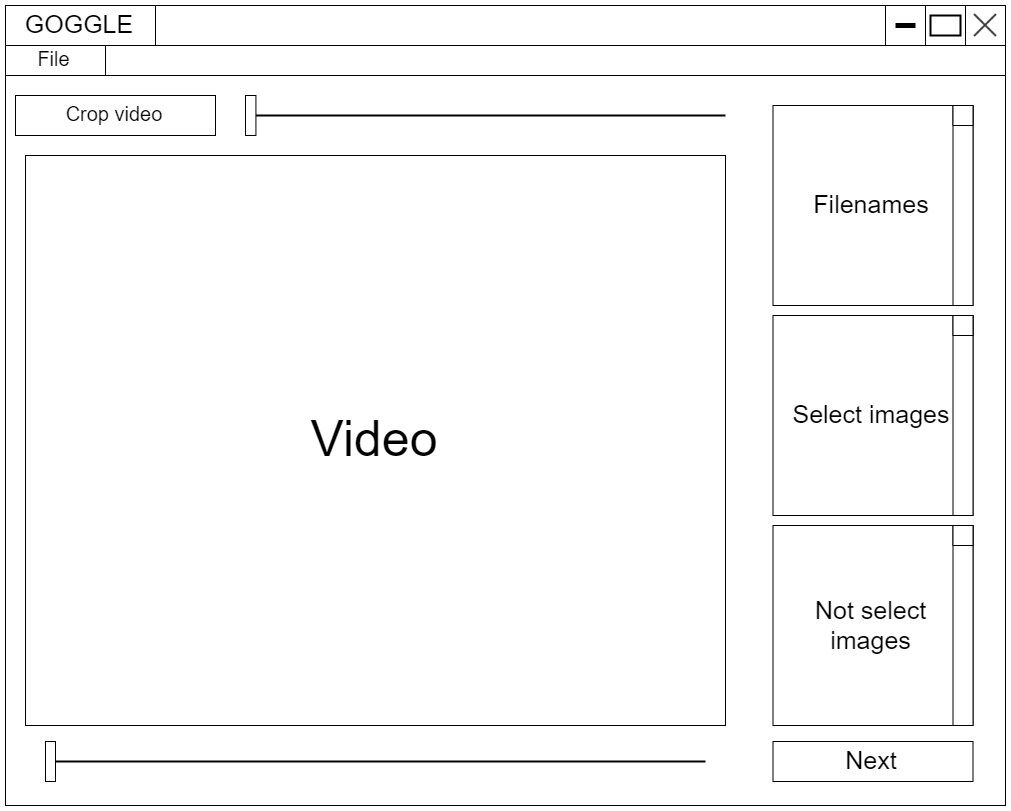
\includegraphics[width=1\textwidth]{chapter3/images/3_6/SelectDraft.png}
    \caption{หน้าต่าง Select ของเครื่องมือสำหรับกำกับข้อมูลด้วยปัญญาประดิษฐ์}
    \label{fig:SelectDraft}
\end{figure}
\clearpage
\begin{figure}[!ht]
    \centering
    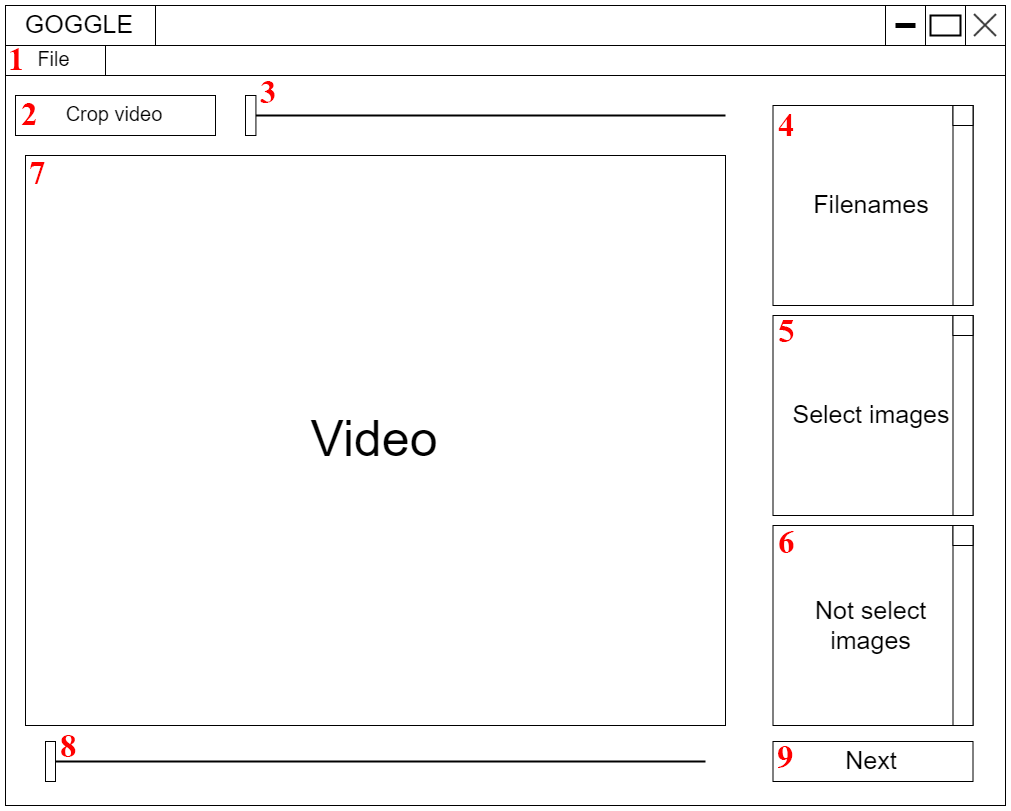
\includegraphics[width=1\textwidth]{chapter3/images/3_6/SelectDraft_point.png}
    \caption{ตำแหน่งของแต่ละวิดเจ็ตในหน้าต่าง Select}
    \label{fig:SelectDraft_point}
\end{figure}
โดยที่แต่ละวิดเจ็ตตามหมายเลขที่กำหนดตามรูปที่ \ref{fig:SelectDraft_point} มีรายละเอียดดังนี้
\begin{enumerate}
	\setlength\itemsep{-0.25em}
	\item หมายเลข 1 คือปุ่มสำหรับเลือกไฟล์วิดีโอที่ต้องการจากในคอมพิวเตอร์เข้ามาในโปรแกรม
    \item หมายเลข 2 คือปุ่มสำหรับสั่งให้ระบบทำการสร้างคีย์เฟรมขึ้นมา แล้วใช้ปัญญาประดิษฐ์ประมวลผลเพื่อแยกว่าคีย์เฟรมไหนมีคนอยู่ และคีย์เฟรมไหนไม่มีคนอยู่แบบอัตโนมัติ
    \item หมายเลข 3 คือแถบเลื่อนเพื่อกำหนดความถี่ในการหยิบคีย์เฟรม โดยจะมีช่วงอยู่ที่ 1 เฟรมต่อวินาที จนถึง อัตราเฟรมต่อวินาทีสูงสุดของวิดีโอที่รับเข้ามา
	\item หมายเลข 4 คือกล่องสำหรับแสดงชื่อวิดีโอที่รับเข้ามาในโปรแกรมเพื่อเลือกเข้ามาใช้ในการประมวลผล
	\item หมายเลข 5 คือกล่องสำหรับแสดงว่าคีย์เฟรมใดมีมนุษย์อยู่ในเฟรม โดยที่ผู้ใช้งานสามารถตรวจสอบความถูกต้องและแก้ไขข้อผิดพลาดของปัญญาประดิษฐ์ได้
	\item หมายเลข 6 คือกล่องสำหรับแสดงว่าคีย์เฟรมใดไม่มีมนุษย์อยู่ในเฟรม โดยที่ผู้ใช้งานสามารถตรวจสอบความถูกต้องและแก้ไขข้อผิดพลาดของปัญญาประดิษฐ์ได้
	\item หมายเลข 7 คือหน้าต่างสำหรับแสดงเฟรมที่เลือกจากหมายเลข 5 หมายเลข 6 หรือหมายเลข 8
	\item หมายเลข 8 คือแถบเลื่อนสำหรับเลื่อนดูคีย์เฟรมทั้งหมดที่ระบบสร้างขึ้น
	\item หมายเลข 9 คือปุ่มสำหรับไปกระบวนการต่อไปหลังจากระบบประมวลผลเสร็จแล้ว
\end{enumerate}
\clearpage

\subsubsection{Detect}
กระบวนการ Delect จะต้องสามารถรับคีย์เฟรมจากกระบวนการ Select มาประมวลผลด้วยปัญญาประดิษฐ์เพื่อหาตำแหน่งของมนุษย์ที่อยู่ในคีย์เฟรม 
แล้วสร้างกรอบสี่เหลี่ยมครอบบริเวณดังกล่าวได้ในแบบอัตโนมัติ เพื่อแบ่งเบาภาระผู้ใช้ในการที่ต้องสร้างกรอบสี่เหลี่ยมครอบตำแหน่งของมนุษย์ด้วยตัวเอง
และผู้ใช้ต้องสามารถสร้างหรือลบกรอบสี่เหลี่ยมได้ด้วยตัวเองสำหรับแก้ไขความผิดพลาดของปัญญาประดิษฐ์ เพื่อเพิ่มคุณภาพของชุดข้อมูล
จึงออกแบบหน้าต่างได้ดังรูปที่ \ref{fig:DetectDraft}
\begin{figure}[!ht]
    \centering
    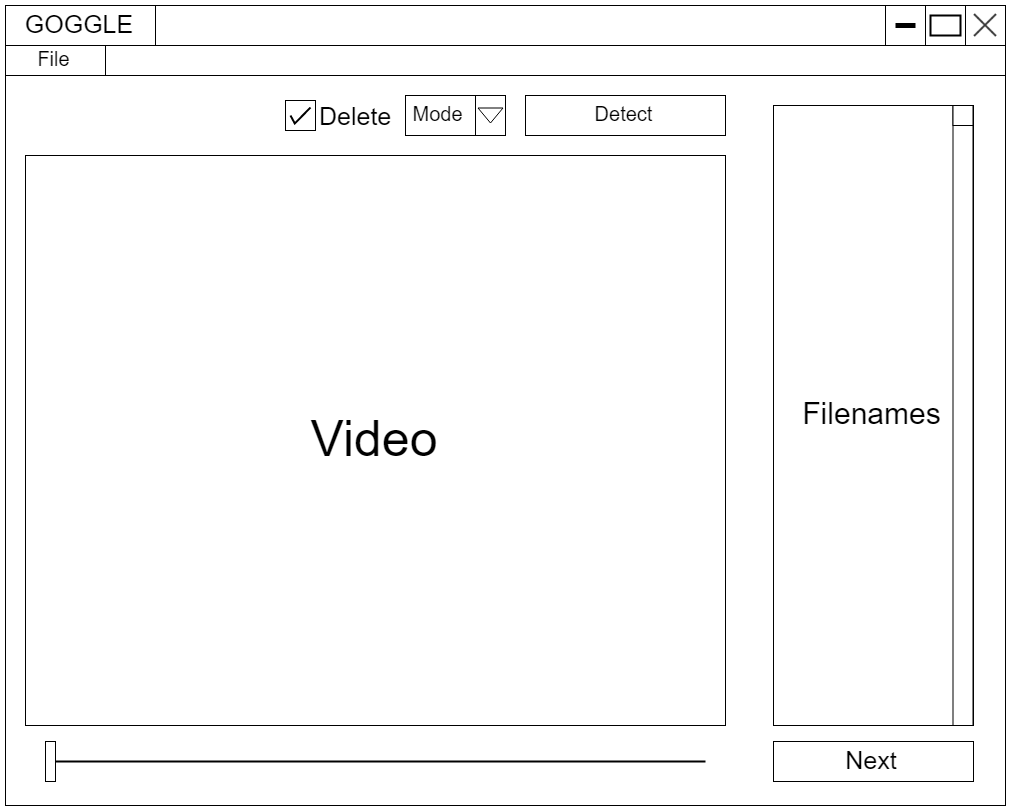
\includegraphics[width=1\textwidth]{chapter3/images/3_6/DetectDraft.png}
    \caption{หน้าต่าง Detect ของเครื่องมือสำหรับกำกับข้อมูลด้วยปัญญาประดิษฐ์}
    \label{fig:DetectDraft}
\end{figure}
\clearpage
\begin{figure}[!ht]
    \centering
    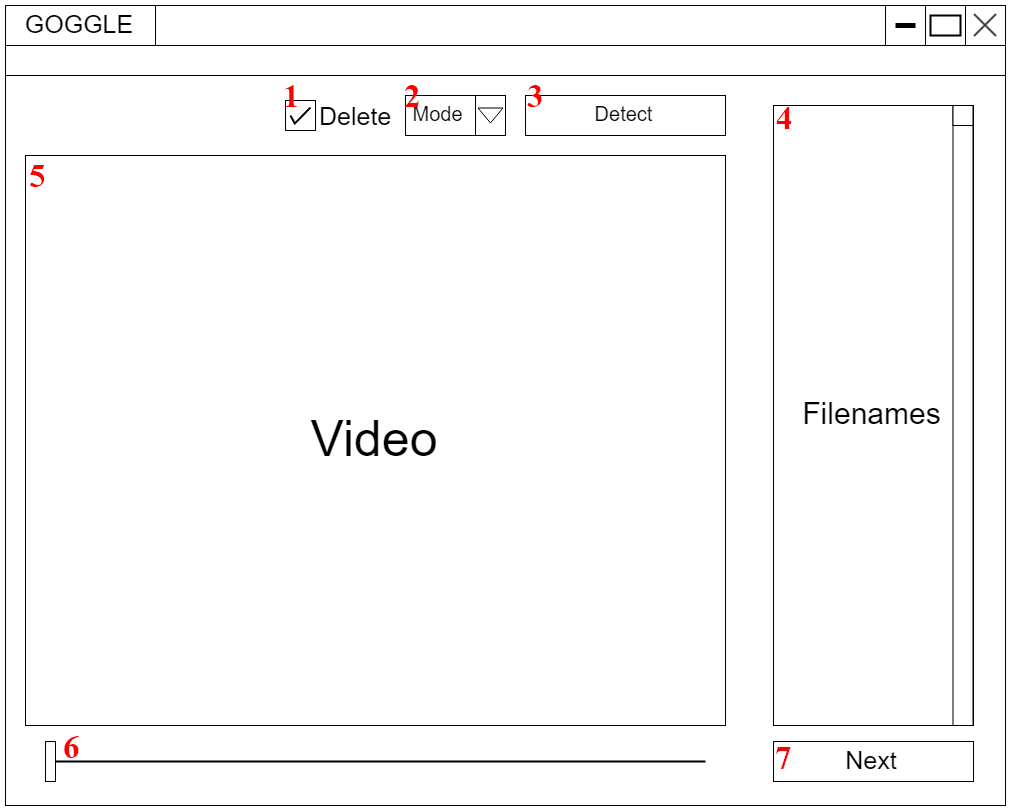
\includegraphics[width=1\textwidth]{chapter3/images/3_6/DetectDraft_point.png}
    \caption{ตำแหน่งของแต่ละวิดเจ็ตในหน้าต่าง Detect}
    \label{fig:DelectDraft_point}
\end{figure}
โดยที่แต่ละวิดเจ็ตตามหมายเลขที่กำหนดตามรูปที่ \ref{fig:DelectDraft_point} มีรายละเอียดดังนี้
\begin{enumerate}
	\setlength\itemsep{-0.25em}
    \item หมายเลข 1 คือช่องสำหรับกดเพื่อเปลี่ยนระบบจากสร้างกรอบสี่เหลี่ยมในแบบแก้ไขด้วยตนเองเป็นลบกรอบสี่เหลี่ยมแทน
    \item หมายเลข 2 คือช่องสำหรับเลือกว่าจะใช้ระบบแบบใด ระหว่างแบบอัตโนมัติและแบบแก้ไขด้วยตนเอง
    \item หมายเลข 3 คือปุ่มสำหรับสั่งให้ระบบทำการตรวจหาตำแหน่งของมนุษย์ในคีย์เฟรมทั้งหมดแล้วสร้างกรอบสี่เหลี่ยมขึ้นมาครอบบริเวณที่กำหนด
	\item หมายเลข 4 คือกล่องสำหรับแสดงคีย์เฟรมทั้งหมด
	\item หมายเลข 5 คือหน้าต่างสำหรับแสดงเฟรมที่เลือกจากหมายเลข 4 หรือหมายเลข 6
	\item หมายเลข 6 คือแถบเลื่อนสำหรับเลื่อนดูคีย์เฟรมทั้งหมดที่มี เพื่อตรวจสอบความถูกต้องของปัญญาประดิษฐ์
	\item หมายเลข 7 คือปุ่มสำหรับไปกระบวนการต่อไปหลังจากระบบประมวลผลเสร็จแล้ว
\end{enumerate}
\clearpage

\subsubsection{Track}
เนื่องจากกระบวนการ Detect นั้นจะทำเฉพาะในคีย์เฟรมทำให้ในเฟรมอื่นๆนอกเหนือจากนั้นจะไม่มีกรอบสี่เหลี่ยมอยู่
ดังนั้นกระบวนการ Track จึงต้องสามารถทำนายตำแหน่งต่อไปของมนุษย์แล้วสร้างกรอบสี่เหลี่ยมขึ้นมาบนเฟรมระหว่างคีย์เฟรมทั้งหมดได้โดยอัตโนมัติ
เพื่อสร้างข้อมูลตำแหน่งของมนุษย์ในเฟรมเหล่านั้น และผู้ใช้ต้องสามารถสร้างหรือลบกรอบสี่เหลี่ยมได้ด้วยตัวเองสำหรับแก้ไขความผิดพลาดของอัลกอริทึม
จึงออกแบบหน้าต่างได้ดังรูปที่ \ref{fig:TrackDraft}
\begin{figure}[!ht]
    \centering
    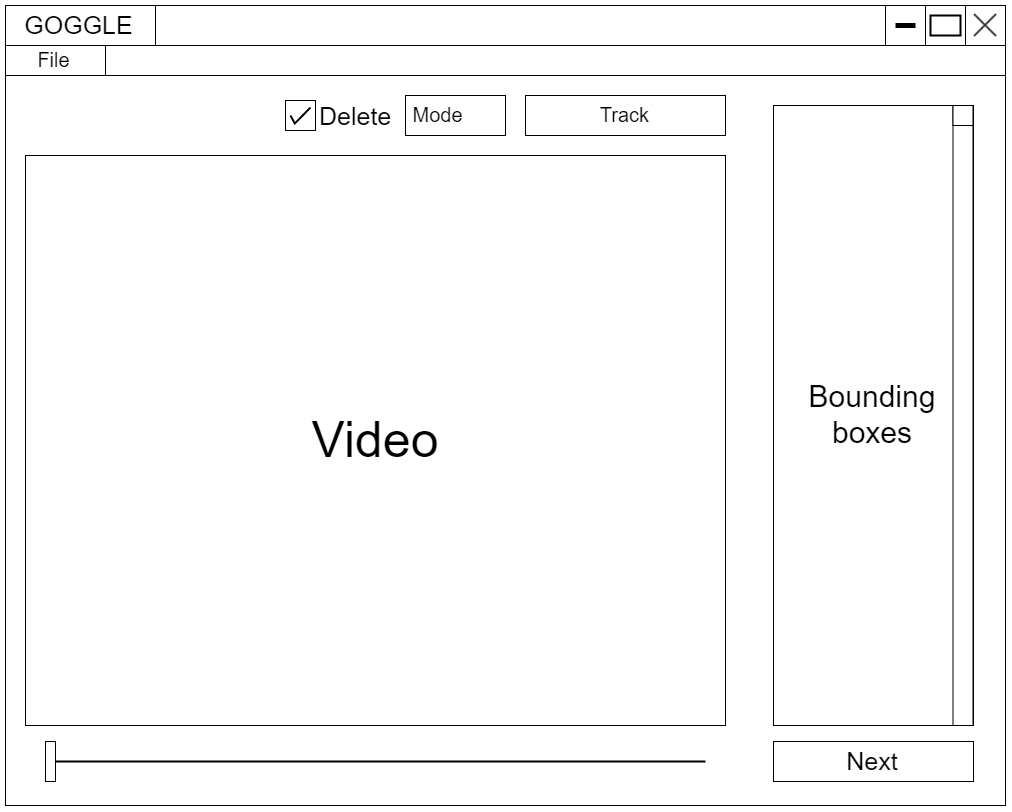
\includegraphics[width=1\textwidth]{chapter3/images/3_6/TrackDraft.png}
    \caption{หน้าต่าง Track ของเครื่องมือสำหรับกำกับข้อมูลด้วยปัญญาประดิษฐ์}
    \label{fig:TrackDraft}
\end{figure}
\clearpage
\begin{figure}[!ht]
    \centering
    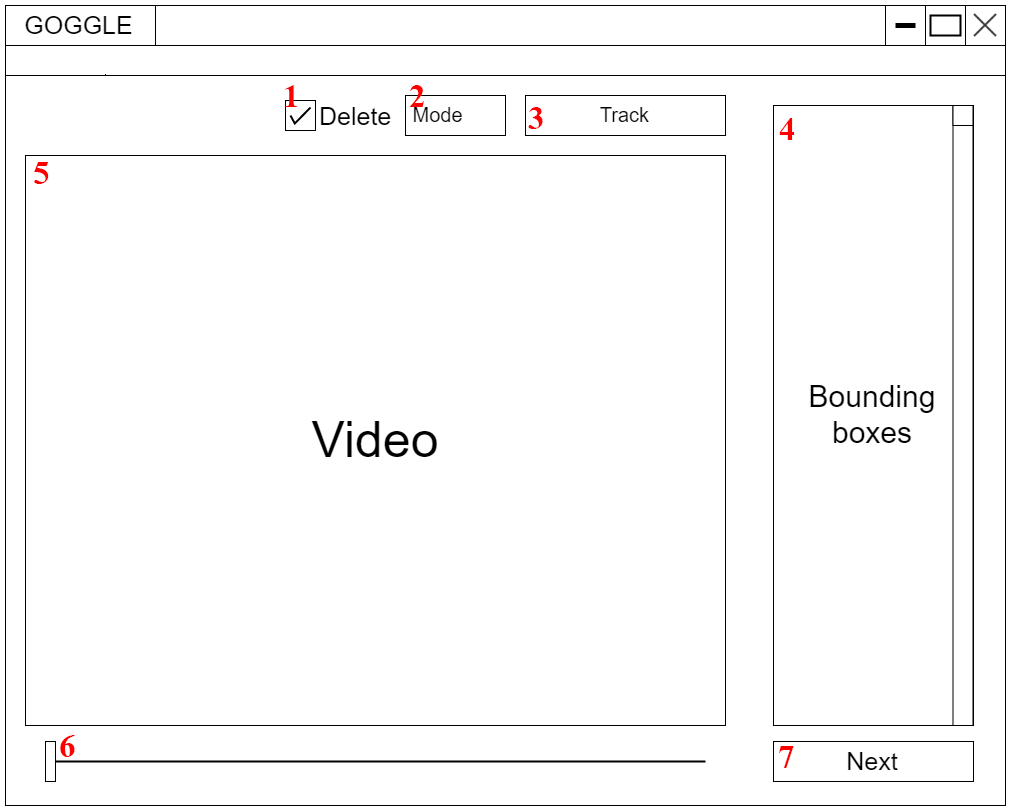
\includegraphics[width=1\textwidth]{chapter3/images/3_6/TrackDraft_point.png}
    \caption{ตำแหน่งของแต่ละวิดเจ็ตในหน้าต่าง Track}
    \label{fig:TrackDraft_point}
\end{figure}
โดยที่แต่ละวิดเจ็ตตามหมายเลขที่กำหนดตามรูปที่ \ref{fig:TrackDraft_point} มีรายละเอียดดังนี้
\begin{enumerate}
	\setlength\itemsep{-0.25em}
    \item หมายเลข 1 คือช่องสำหรับกดเพื่อเปลี่ยนระบบจากสร้างกรอบสี่เหลี่ยมในแบบแก้ไขด้วยตนเองเป็นลบกรอบสี่เหลี่ยมแทน
    \item หมายเลข 2 คือช่องสำหรับเลือกว่าจะใช้ระบบแบบใด ระหว่างแบบอัตโนมัติและแบบแก้ไขด้วยตนเอง
    \item หมายเลข 3 คือปุ่มสำหรับสั่งให้ระบบทำการตรวจหาตำแหน่งของมนุษย์ในเฟรมระหว่างคีย์เฟรมทั้งหมดแล้วสร้างกรอบสี่เหลี่ยมขึ้นมาครอบบริเวณที่กำหนด
	\item หมายเลข 4 คือกล่องสำหรับแสดงกรอบสี่เหลี่ยมทั้งหมดที่อยู่ในเฟรม
	\item หมายเลข 5 คือหน้าต่างสำหรับแสดงเฟรมที่เลือกจากหมายเลข 6
	\item หมายเลข 6 คือแถบเลื่อนสำหรับเลื่อนดูเฟรมทั้งหมดที่มี เพื่อตรวจสอบความถูกต้องของอัลกอริทึม
	\item หมายเลข 7 คือปุ่มสำหรับไปกระบวนการต่อไปหลังจากระบบประมวลผลเสร็จแล้ว
\end{enumerate}
\clearpage

\subsubsection{Label}
กระบวนการ Label นั้นต้องสามารถทำนายว่าการกระทำของมนุษย์ที่อยู่ในแต่ละเฟรมว่าคืออะไรได้โดยอัตโนมัติด้วยปัญญาประดิษฐ์
และผู้ใช้จะต้องสามารถแก้ไขข้อผิดพลาดของปัญญาประดิษฐ์ได้หากมีการทำนายที่ผิดพลาดเกิดขึ้น
หรือถ้าหากผู้ใช้ต้องการเพิ่มการกระทำที่ไม่ได้มีอยู่ในชุดการกระทำพื้นฐานที่มีอยู่แล้วของปัญญาประดิษฐ์ ผู้ใช้ก็สามารถเพิ่มการกระทำนั้นเข้ามาได้
จึงออกแบบหน้าต่างได้ดังรูปที่ \ref{fig:ActionLabelDraft}
\begin{figure}[!ht]
    \centering
    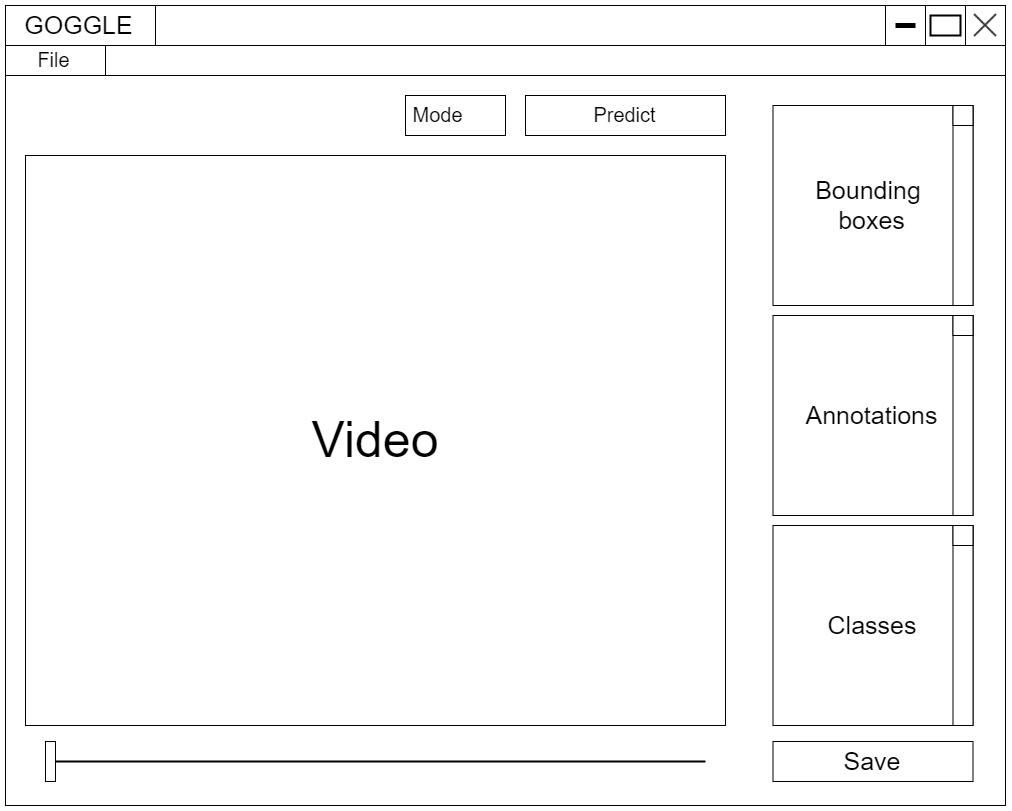
\includegraphics[width=1\textwidth]{chapter3/images/3_6/ActionLabelDraft.png}
    \caption{หน้าต่าง Label ของเครื่องมือสำหรับกำกับข้อมูลด้วยปัญญาประดิษฐ์}
    \label{fig:ActionLabelDraft}
\end{figure}
\clearpage
\begin{figure}[!ht]
    \centering
    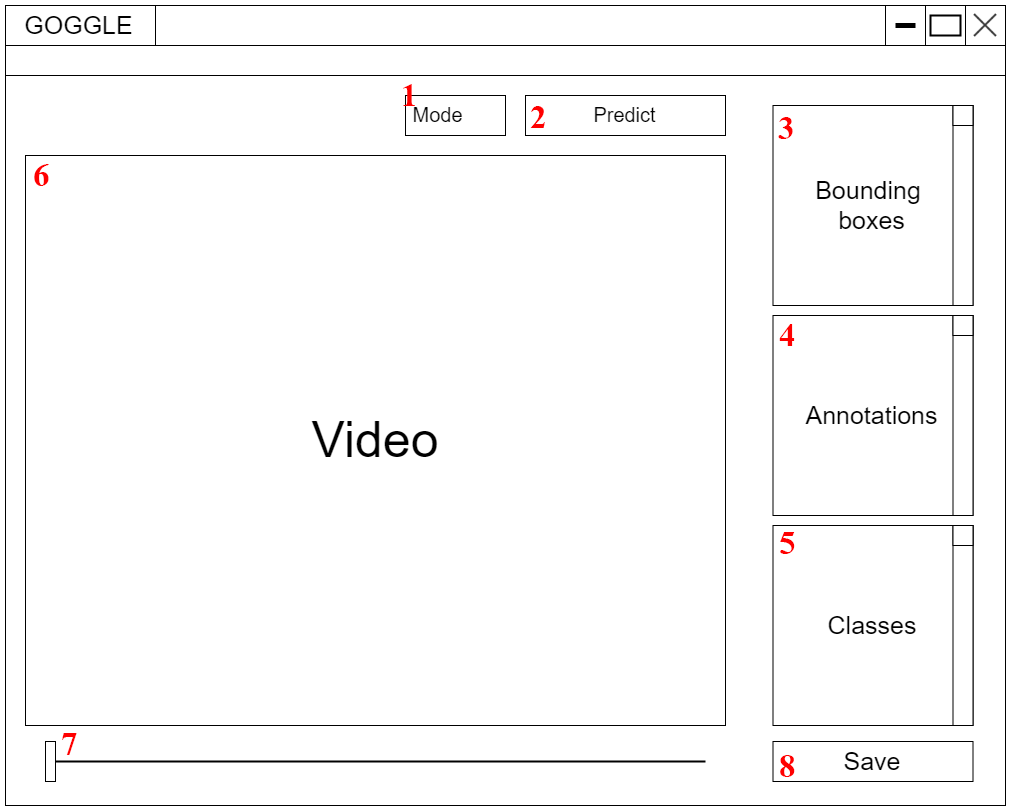
\includegraphics[width=1\textwidth]{chapter3/images/3_6/ActionLabelDraft_point.png}
    \caption{ตำแหน่งของแต่ละวิดเจ็ตในหน้าต่าง Label}
    \label{fig:ActiobLabelDraft_point}
\end{figure}
โดยที่แต่ละวิดเจ็ตตามหมายเลขที่กำหนดตามรูปที่ \ref{fig:TrackDraft_point} มีรายละเอียดดังนี้
\begin{enumerate}
	\setlength\itemsep{-0.25em}
    \item หมายเลข 1 คือช่องสำหรับเลือกว่าจะใช้ระบบแบบใด ระหว่างแบบอัตโนมัติและแบบแก้ไขด้วยตนเอง
    \item หมายเลข 2 คือปุ่มสำหรับสั่งให้ระบบทำนายการกระทำของมนุษย์ในทุกๆเฟรม
    \item หมายเลข 3 คือกล่องสำหรับแสดงกรอบสี่เหลี่ยมทั้งหมดที่อยู่ในเฟรมที่เลือก
	\item หมายเลข 4 คือกล่องสำหรับแสดงการกระทำของมนุษย์แต่ละคนที่อยู่ในเฟรมที่เลือก โดยจะเรียงลำดับคู่กับกรอบสี่เหลี่ยมที่อยู่ในช่องหมายเลข 3
    \item หมายเลข 5 คือกล่องสำหรับแสดงชุดการกระทำที่ปัญญาประดิษฐ์มีอยู่แล้ว ซึ่งในการทำงานแบบแก้ไขด้วยตนเองนั้น จะสามารถค้นหาการกระทำที่มีอยู่แล้วได้ 
    และหากคำที่ใส่เข้ามานั้นไม่มีอยู่ในชุดการกระทำก็จะเป็นการเพิ่มการกระทำนั้นเข้ามาแทน
	\item หมายเลข 6 คือหน้าต่างสำหรับแสดงเฟรมที่เลือกจากหมายเลข 7
	\item หมายเลข 7 คือแถบเลื่อนสำหรับเลื่อนดูเฟรมทั้งหมดที่มี เพื่อตรวจสอบความถูกต้องของปัญญาประดิษฐ์
	\item หมายเลข 8 คือปุ่มสำหรับสร้างไฟล์ xml ของทุกๆเฟรมสำหรับใช้ในการสร้างโมเดลโดยรายละเอียดข้อมูลภายในไฟล์ xml จะอยู่ในหัวข้อ \ref{sec:XMLInfo}
\end{enumerate}
\clearpage

\subsubsection{รายละเอียดข้อมูลภายในไฟล์ xml}
\label{sec:XMLInfo}
ไฟล์ xml นั้นเป็นรูปแบบที่นิยมใช้ในการเก็บข้อมูลสำหรับการสร้างโมเดลประเภทตรวจจับวัตถุ
โดยจะเก็บข้อมูลในรูปแบบของ PASCAL VOC ที่นิยมใช้ในการสร้างโมเดลด้วย Tensorflow โดยภายในไฟล์จะมีข้อมูลดังรูปที่ \ref{fig:XMLFormat}
\begin{figure}[!ht]
    \centering
    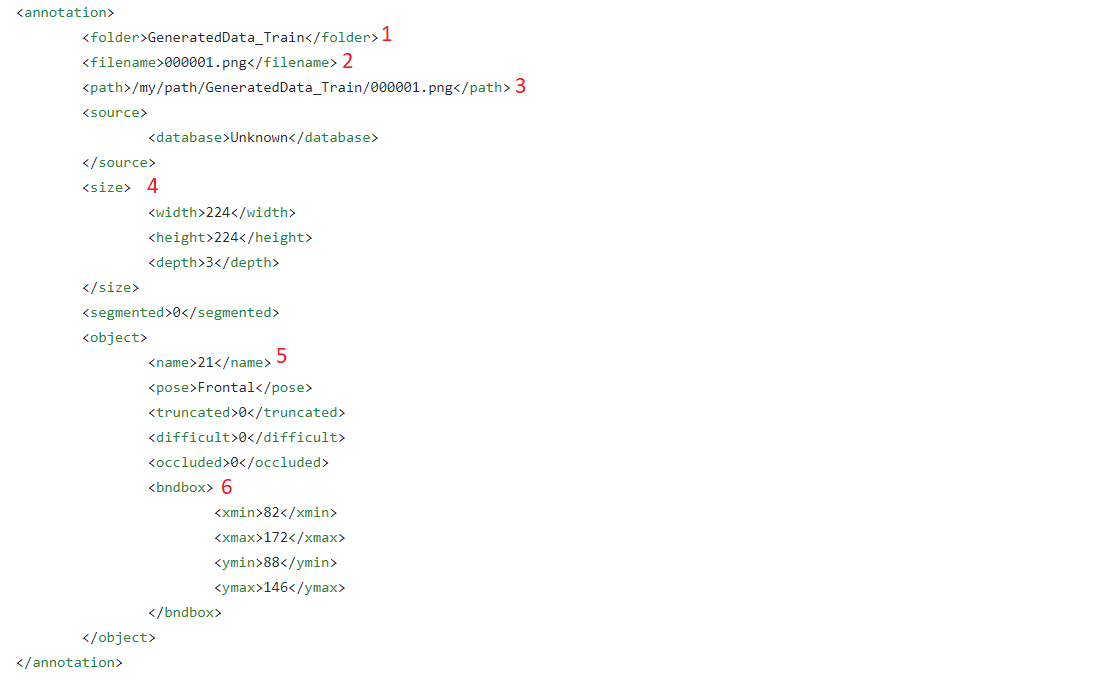
\includegraphics[width=1\textwidth]{chapter3/images/3_6/XMLFormat.png}
    \caption{ตัวอย่างข้อมูลภายในไฟล์ xml}
    \label{fig:XMLFormat}
\end{figure}
โดยข้อมูลส่วนสำคัญของรูปแบบนี้นั้นจะถูกใส่หมายเลขกำกับไว้ซึ่งแต่ละหมายเลขนั้นหมายถึง
\begin{enumerate}
	\setlength\itemsep{-0.25em}
    \item หมายเลข 1 คือชื่อโฟลเดอร์ที่เก็บไฟล์รูปภาพที่เกี่ยวข้องกับไฟล์ xml นี้อยู่
    \item หมายเลข 2 คือชื่อไฟล์ที่เกี่ยวข้องกับไฟล์ xml นี้
    \item หมายเลข 3 คือเส้นทางในคอมพิวเตอร์ (directory path) ของไฟล์รูปภาพที่เกี่ยวข้องกับไฟล์ xml นี้
    \item หมายเลข 4 คือขนาดและมิติของรูปภาพ ซึ่งจะประกอบด้วยความกว้าง (width) ความยาว (height) และจำนวนช่องสี (depth) 
    โดยที่จำนวนช่องสีที่มีความลึก 3 มักจะหมายถึงภาพสี RGB และจำนวนช่องสีที่มีความลึก 2 จะหมายถึงภาพขาวดำ (gray scale)
	\item หมายเลข 5 คือ label ของวัตถุหรืออย่างอื่น ที่อยู่ในกรอบสี่เหลี่ยมที่ถูกกำหนดไว้ในส่วนของหมายเลข 6
	\item หมายเลข 6 คือ กรอบสี่เหลี่ยมที่ครอบวัตถุที่สนใจ เช่นมนุษย์ เป็นต้น
\end{enumerate}
\clearpage

\section{การออกแบบการทดสอบการตรวจจับวัตถุ}
\subsection{ทดสอบประสิทธิภาพการทำงานของโมเดลปัญญาประดิษฐ์สำหรับการทำการตรวจจับภาพบุคคล}
\subsection*{สิ่งที่ใช้ในการวัดผล}
	\begin{enumerate}
		\setlength\itemsep{-0.25em}
		\item ความเร็วในการทำนายต่อรูปภาพ (มิลลิวินาที)
		\item ความแม่นยำ โดยคำนึงถึงอัตราส่วนร่วมของกรอบที่เหลี่ยม หรือ Intersection over Union (IoU)
	\end{enumerate}
\subsection*{จุดประสงค์}
	\begin{enumerate}
		\setlength\itemsep{-0.25em}
		\item ผู้วิจัยได้ตั้งจุดประสงค์การทดลองการใช้โมเดลปัญญาประดิษฐ์สำหรับตรวจจับวัตถุ เพื่อวัดผลโมเดลปัญญาประดิษฐ์ที่ใช้ในปัจจุบัน
และหาโมเดลปัญญาประดิษฐ์สำหรับการตรวจจับวัตถุที่มีความเร็วมากที่สุดและแม่นยำสูงที่สุดเมื่อทดสอบกับชุดข้อมูลของผู้วิจัย
	\end{enumerate}
\subsection*{ตัวแปร}
	\begin{enumerate}
		\setlength\itemsep{-0.25em}
		\item โมเดลปัญญาประดิษฐ์ ได้แก่
		\begin{enumerate}
			\setlength\itemsep{-0.25em}
			\item SSD Mobilenet v1 ppn
			\item YOLO-v3 tiny
			\item YOLO-v3 spp	
			\item YOLO-v3 320
			\item Faster RCNN inception v2
		\end{enumerate}
	\end{enumerate}
\subsection*{ตัวแปรควบคุม}
	\begin{enumerate}
		\setlength\itemsep{-0.25em}
		\item ชุดข้อมูล : ชุดข้อมูลสำหรับทดสอบวัดผลที่ผู้วิจัยสร้างขึ้น (สุ่ม 20 เฟรมจากวิดีโอที่ผู้วิจัยใช้สำหรับสร้างชุดข้อมูล)
	\end{enumerate}
\subsection*{วิธีการทดลอง}
	\begin{enumerate}
		\setlength\itemsep{-0.25em}
		\item แบ่งชุดข้อมูลออกเป็นชุดข้อมูลสำหรับทดสอบ และชุดข้อมูลที่มีคำกำกับเพื่อเป็นคำตอบ
			\begin{enumerate}
				\setlength\itemsep{-0.25em}
				\item ชุดข้อมูลสำหรับทดสอบ ประกอบด้วย : ชื่อของวิดีโอ และเฟรม
				\item ชุดข้อมูลที่มีคำกำกับเพื่อเป็นคำตอบ ประกอบด้วย : ชื่อของวิดีโอ เฟรม และตำแหน่งของกรอบสี่เหลี่ยม
			\end{enumerate}
		\item เรียกชื่อและเฟรมของวิดีโอจากชุดข้อมูลทดสอบ และนำโมเดลปัญญาประดิษฐ์ทำนายผลลัพธ์ จากนั้นเก็บผลลัพธ์เป็นชุดข้อมูลผลลัพธ์จากการทำนาย
			\begin{enumerate}
				\setlength\itemsep{-0.25em}
				\item ชุดข้อมูลผลลัพธ์จากการทำนาย ประกอบด้วย : ชื่อของวิดีโอ เฟรม และตำแหน่งของกรอบสี่เหลี่ยม
			\end{enumerate}
		\item ประเมินผลค่าความแม่นยำในการทำงานโดยเทียบระหว่างชุดผลลัพธ์จากการทำนาย และชุดข้อมูลที่มีคำกำกับเพื่อเป็นคำตอบ โดยกำหนดให้ค่า IoU >= 0.5	จึงจะนับว่าทำนายได้ถูก
		\item เปรียบเทียบผลลัพธ์จากแหล่งที่มา
\end{enumerate}

\clearpage

\section{การออกแบบการทดสอบการทำนายตำแหน่งต่อไปของมนุษย์}
\subsection{ทดสอบประสิทธิภาพการทำงานของระบบทำนายตำแหน่งต่อไปของวัตถุในวิดีโอ}
\subsection*{สิ่งที่ใช้ในการวัดผล}
	\begin{enumerate}
		\item ความเร็วในการทำนายต่อวิดีโอ (วินาที)
		\item ความแม่นยำ โดยคำนึงถึงอัตราส่วนร่วมของกรอบที่เหลี่ยม
	\end{enumerate}
\subsection*{สมมุติฐาน}
ผู้วิจัยได้ตั้งสมมุติฐานว่า การใช้โมเดลปัญญาประดิษฐ์สำหรับตรวจจับวัตถุและสร้างกรอบสี่เหลี่ยมทุกๆ N เฟรม 
แล้วใช้ระบบทำนายตำแหน่งต่อไปของวัตถุในการสร้างกรอบสี่เหลี่ยมในเฟรมระหว่างนั้น จะทำให้ระบบสามารถทำงานได้เร็วขึ้น โดยที่ประสิทธิภาพจะลดลงเพียงเล็กน้อย
\subsection*{ตัวแปรควบคุม}
	\begin{enumerate}
		\item วิดีโอสาธารณะที่ไม่ติดลิขสิทธิ์ ความยาวประมาณ 10 - 30 วินาที หนึ่งวิดีโอ
		\item ใช้โมเดลปัญญาประดิษฐ์สำหรับตรวจจับตำแหน่งวัตถุ ResNet50 ในการสร้างชุดข้อมูลที่มีการกำกับตำแหน่งวัตถุไว้ (ground-truth) แล้วใช้มนุษย์ในการตรวจสอบความถูกต้อง
		เพื่อใช้เป็นคำตอบของการทำนาย
		\item โมเดลปัญญาประดิษฐ์สำหรับตรวจจับตำแหน่งที่ใช้ในการเปรียบเทียบ: YOLO-V3 320
		\item อัลกอริทึมสำหรับระบบทำนายตำแหน่งต่อไปของวัตถุ: dlib
		\item อัตราส่วนร่วมของกรอบที่เหลี่ยม: มีส่วนที่ทับกันมากกว่า 80\% ขึ้นไปจึงจะนับว่าผลการทำนายถูกต้อง
	\end{enumerate}
\subsection*{วิธีการทดลอง}
	\begin{enumerate}
		\item ใช้โมเดลปัญญาประดิษฐ์ YOLO-v3 320 ประมวลผลทุกเฟรมในวิดีโอ และเปรียบเทียบผลลัพธ์กับชุดข้อมูลที่ถูกกำกับตำแหน่งวัตถุไว้แล้ว เพื่อคำนวณหาความแม่นยำ
		\item ใช้โมเดลปัญญาประดิษฐ์ YOLO-v3 320 ประมวลผลทุกๆ N เฟรมในวิดีโอ แล้วใช้ระบบทำนายตำแหน่งต่อไปของวัตถุในการสร้างกรอบสี่เหลี่ยมในเฟรมระหว่างนั้น 
		และเปรียบเทียบผลลัพธ์กับชุดข้อมูลที่ถูกกำกับตำแหน่งวัตถุไว้แล้ว เพื่อคำนวณหาความแม่นยำ โดยที่ค่า N จะเท่ากับ 10 20 และ 25
		\item เปรียบเทียบความเร็วในการประมวลผล และความแม่นยำ
\end{enumerate}
\clearpage

\section{การออกแบบการทดสอบการระบุตัวตนของมนุษย์}
\subsection{ทดสอบประสิทธิภาพการทำงานของระบบระบุตัวตนของบุคคลภายในภาพ}
\subsection*{สิ่งที่ใช้ในการวัดผล}
	\begin{enumerate}
		\setlength\itemsep{-0.25em}
		\item ค่า AUC ที่ใช้สำหรับการระบุตัวตนของบุคคลภายในภาพ
	\end{enumerate}
\subsection*{สมมติฐาน}
ผู้วิจัยได้ตั้งสมมติฐานว่า ผลลัพธ์ของการทดลองการใช้งานจริงของโมเดลปัญญาประดิษฐ์ ResNet50 ที่สร้างด้วยชุดข้อมูล Market1501 
นั้นควรจะมีความแม่นยำในการระบุตัวตนของบุคคลภายในภาพมากที่สุดเมื่อเทียบกับโมเดลปัญญาประดิษฐ์ที่สร้างด้วยชุดข้อมูลอื่นๆ
เพราะเมื่อเทียบกับโมเดลปัญญาประดิษฐ์ที่ถูกสร้างด้วยชุดข้อมูลอื่นที่มาจากแหล่งข้อมูลเดียวกัน โมเดลปัญญาประดิษฐ์ ResNet50 ที่สร้างด้วยชุดข้อมูล Market1501 นั้นจะมีความแม่นยำสูงสุด
\subsection*{ตัวแปร}
	\begin{enumerate}
		\setlength\itemsep{-0.25em}
		\item โมเดลปัญญาประดิษฐ์ ซึ่งได้แก่
		\begin{enumerate}
			\setlength\itemsep{-0.25em}
			\item ResNet50 ที่ถูกสร้างด้วยชุดข้อมูล Market1501
			\item ResNet50 ที่ถูกสร้างด้วยชุดข้อมูล DukeMTMCReID
			\item ResNet50 ที่ถูกสร้างด้วยชุดข้อมูล CUHK03	
			\item ResNet50 ที่ถูกสร้างด้วยชุดข้อมูล MSMT17
		\end{enumerate}
	\end{enumerate}
\subsection*{ตัวแปรควบคุม}
	\begin{enumerate}
		\setlength\itemsep{-0.25em}
		\item ชุดข้อมูล : ชุดข้อมูลที่ทางผู้วิจัยสร้างขึ้นสำหรับการทดสอบ
		\item โมเดลปัญญาประดิษฐ์ : YOLO-V3 320  สำหรับการหาตำแหน่งของบุคคล
	\end{enumerate}
\subsection*{วิธีการทดลอง}
	\begin{enumerate}
		\setlength\itemsep{-0.25em}
		\item นำชุดข้อมูลที่ผู้วิจัยสร้างขึ้นมาผ่านโมเดลปัญญาประดิษฐ์ YOLO-V3 320 เพื่อหาตำแหน่งของบุคคล
		\item นำโมเดลปัญญาประดิษฐ์แต่ละอันมาทดสอบความแม่นยำสำหรับการระบุตัวตนของบุคคลภายในภาพ ด้วยตำแหน่งของบุคคลที่ได้มาจากขั้นตอนก่อนหน้านี้
		\item ประเมินผลการทำงานโดยเทียบค่า AUC สำหรับการระบุตัวตนของบุคคลภายในภาพของแต่ละโมเดลปัญญาประดิษฐ์ เพื่อหาโมเดลปัญญาประดิษฐ์ที่เหมาะสมกับชุดข้อมูลของผู้วิจัยมากที่สุด
\end{enumerate}

\clearpage

\section{การออกแบบการทดสอบการจดจำการกระทำของมนุษย์}
\subsection{ทดสอบประสิทธิภาพการทำงานของโมเดลปัญญาประดิษฐ์ที่เคยถูกเทรนด์ผ่าน AVA โดยใช้ชุดข้อมูลของ AVA ในการทดสอบและเทียบผลลัพธ์กับแหล่งอ้างอิง}
\subsection*{สิ่งที่ใช้ในการวัดผล}
	\begin{enumerate}
		\setlength\itemsep{-0.25em}
		\item ความเร็วในการทำนายต่อรูปภาพ (มิลลิวินาที)
		\item ความแม่นยำ (PASCAL mAP)
	\end{enumerate}
\subsection*{สมมุติฐาน}
ผู้วิจัยได้ตั้งสมมุติฐานว่า ผลลัพธ์ของการทดลองจะมีความแม่นยำเทียบเท่ากับผลลัพธ์จากแหล่งที่มา แต่ความเร็วต่อรูปภาพจะมีความเร็วน้อยกว่าผลลัพธ์จากแหล่งที่มา 
เนื่องจากแหล่งที่มาของข้อมูลได้ทำการทดสอบโดยใช้กราฟิกการ์ดรุ่น Nvidia GeForce GTX TITAN X ซึ่งเป็นกราฟิกการ์ดที่มีประสิทธิภาพการทำงานดีกว่ากราฟิกการ์ดของผู้วิจัย จึงทำให้สามารถทดสอบด้วยความเร็วที่มากกว่า
\subsection*{ตัวแปรควบคุม}
	\begin{enumerate}
		\setlength\itemsep{-0.25em}
		\item ชุดข้อมูล : The validation split of AVA v2.1
		\item โมเดลปัญญาประดิษฐ์ : Faster RCNN ResNet101 AVA v2.1
	\end{enumerate}
\subsection*{วิธีการทดลอง}
	\begin{enumerate}
		\setlength\itemsep{-0.25em}
		\item ดาวน์โหลดชุดข้อมูล The validation split of AVA v2.1
		\item แบ่งชุดข้อมูลออกเป็น ชุดข้อมูลสำหรับทดสอบ และชุดข้อมูลที่มีคำกำกับเพื่อเป็นคำตอบ
			\begin{enumerate}
				\setlength\itemsep{-0.25em}
				\item ชุดข้อมูลสำหรับทดสอบ ประกอบด้วย : ชื่อของวิดีโอ
				\item ชุดข้อมูลที่มีคำกำกับเพื่อเป็นคำตอบ ประกอบด้วย : ชื่อของวิดีโอ เฟรม ตำแหน่งของกรอบสี่เหลี่ยม และรหัสของการกระทำ
			\end{enumerate}
		\item เรียกชื่อของวิดีโอจากชุดข้อมูลทดสอบ และนำโมเดลปัญญาประดิษฐ์ทำนายผลลัพธ์ จากนั้นเก็บผลลัพธ์เป็นชุดข้อมูลผลลัพธ์จากการทำนาย
			\begin{enumerate}
				\setlength\itemsep{-0.25em}
				\item ชุดข้อมูลผลลัพธ์จากการทำนาย ประกอบด้วย : ชื่อของวิดีโอ เฟรม ตำแหน่งของกรอบสี่เหลี่ยม รหัสของการกระทำ และความมั่นใจ
			\end{enumerate}
		\item ประเมินผลการทำงานโดยเทียบระหว่างชุดผลลัพธ์จากการทำนาย และชุดข้อมูลที่มีคำกำกับเพื่อเป็นคำตอบ
		\item เปรียบเทียบผลลัพธ์จากแหล่งที่มา
\end{enumerate}
\clearpage
\subsection{ทดสอบประสิทธิภาพการทำงานของโมเดลปัญญาประดิษฐ์ที่เคยถูกสร้างด้วย AVA และใช้ชุดข้อมูลที่ผู้วิจัยสร้างขึ้นในการทดสอบและเทียบผลลัพธ์กับแหล่งอ้างอิง}
\subsection*{สิ่งที่ใช้ในการวัดผล}
	\begin{enumerate}
		\setlength\itemsep{-0.25em}
		\item ความในการทำนายเร็วต่อรูปภาพ (มิลลิวินาที)
		\item ความแม่นยำ (PASCAL mAP)
	\end{enumerate}
\subsection*{สมมุติฐาน}ผู้วิจัยได้ตั้งสมมุติฐานว่าผลลัพธ์ของการทดลองจะมีความแม่นยำต่ำลงเมื่อเทียบกับความแม่นยำของการทดลองที่ผ่านมา เนื่องจากชุดข้อมูลที่ผู้วิจัยสร้างขึ้น ได้มีการตัดหมวดหมู่บางอย่างออกไป 
ทำให้โมเดลปัญญาประดิษฐ์ที่ถูกสร้างด้วย AVA มีหมวดหมู่ของการกระทำไม่ตรงกับชุดข้อมูลที่ผู้วิจัยสร้างขึ้น ซึ่งมีผลทำให้ความแม่นยำลดลง ในส่วนของความเร็วต่อรูปภาพจะมีความเร็วน้อยกว่าผลลัพธ์จากแหล่งที่มา เนื่องจาก แหล่งที่มาของข้อมูลได้ทำการทดสอบโดยใช้กราฟิกการ์ดรุ่น Nvidia GeForce GTX TITAN X card ซึ่งเป็นกราฟิกการ์ดที่มีประสิทธิภาพการทำงานดีกว่า กราฟิกการ์ดของผู้วิจัย จึงทำให้สามารถทดสอบด้วยความเร็วที่มากกว่า
\subsection*{ตัวแปรควบคุม}
	\begin{enumerate}
		\setlength\itemsep{-0.25em}
		\item ชุดข้อมูล : ชุดข้อมูลที่ผู้วิจัยสร้างด้วยเครื่องมือกำกับคุณลักษณะ
		\item โมเดลปัญญาประดิษฐ์ : Faster RCNN ResNet101 AVA v2.1
	\end{enumerate}
\subsection*{วิธีการทดลอง}
	\begin{enumerate}
		\setlength\itemsep{-0.25em}
		\item แบ่งชุดข้อมูลออกเป็น ชุดข้อมูลสำหรับทดสอบ และชุดข้อมูลที่มีคำกำกับเพื่อเป็นคำตอบ
			\begin{enumerate}
				\setlength\itemsep{-0.25em}
				\item ชุดข้อมูลสำหรับทดสอบ ประกอบด้วย : ชื่อของวิดีโอ
				\item ชุดข้อมูลที่มีคำกำกับเพื่อเป็นคำตอบ ประกอบด้วย : ชื่อของวิดีโอ เฟรม ตำแหน่งของกรอบสี่เหลี่ยม และรหัสของการกระทำ
			\end{enumerate}
		\item เรียกชื่อของวิดีโอจากชุดข้อมูลทดสอบ และนำโมเดลปัญญาประดิษฐ์ทำนายผลลัพธ์ จากนั้นเก็บผลลัพธ์เป็นชุดข้อมูลผลลัพธ์จากการทำนาย
			\begin{enumerate}
				\setlength\itemsep{-0.25em}
				\item ชุดข้อมูลผลลัพธ์จากการทำนาย ประกอบด้วย : ชื่อของวิดีโอ เฟรม ตำแหน่งของกรอบสี่เหลี่ยม รหัสของการกระทำ และความมั่นใจ
			\end{enumerate}
		\item ประเมินผลการทำงานโดยเทียบระหว่างชุดผลลัพธ์จากการทำนาย และชุดข้อมูลที่มีคำกำกับเพื่อเป็นคำตอบ	
		\item เปรียบเทียบผลลัพธ์กับผลการทดลองที่ผ่านมา
\end{enumerate}
\clearpage
\subsection{ทดสอบประสิทธิภาพการทำงานของโมเดลปัญญาประดิษฐ์ที่ถูกสร้างด้วยชุดข้อมูลที่ผู้วิจัยสร้างขึ้น และใช้ชุดข้อมูลที่ผู้วิจัยสร้างขึ้นในการทดสอบและเทียบผลลัพธ์กับแหล่งอ้างอิง}
\subsection*{สิ่งที่ใช้ในการวัดผล}
	\begin{enumerate}
		\setlength\itemsep{-0.25em}
		\item ความเร็วในการทำนายต่อรูปภาพ (มิลลิวินาที)
		\item ความแม่นยำ (PASCAL mAP)
	\end{enumerate}
\subsection*{สมมุติฐาน}ผู้วิจัยได้ตั้งสมมุติฐานว่าผลลัพธ์ของการทดลองจะมีความแม่นยำสูงขึ้นเมื่อเทียบกับความแม่นยำของการทดลองที่ผ่านมา เนื่องจากโมเดลปัญญาประดิษฐ์ในการทดลองนี้ 
เป็นโมเดลปัญญาประดิษฐ์ที่ผู้วิจัยได้สร้างขึ้น ซึ่งจะมีหมวดหมู่ของการกระทำของโมเดลปัญญาประดิษฐ์และชุดข้อมูลทดสอบตรงกัน ในส่วนของความเร็วต่อรูปภาพจะมีความเร็วน้อยกว่าผลลัพธ์จากแหล่งที่มา 
เนื่องจากแหล่งที่มาของข้อมูลได้ทำการทดสอบโดยใช้กราฟิกการ์ดรุ่น Nvidia GeForce GTX TITAN X ซึ่งเป็นกราฟิกการ์ดที่มีประสิทธิภาพการทำงานดีกว่ากราฟิกการ์ดของผู้วิจัย จึงทำให้สามารถทดสอบด้วยความเร็วที่มากกว่า
\subsection*{ตัวแปรควบคุม}
	\begin{enumerate}
		\setlength\itemsep{-0.25em}
		\item ชุดข้อมูล : ชุดข้อมูลที่ผู้วิจัยสร้างด้วยเครื่องมือกำกับคุณลักษณะ
		\item โมเดลปัญญาประดิษฐ์ : โมเดลปัญญาประดิษฐ์ที่ผู้วิจัยสร้างขึ้น
	\end{enumerate}
\subsection*{วิธีการทดลอง}
	\begin{enumerate}
		\setlength\itemsep{-0.25em}
		\item แบ่งชุดข้อมูลออกเป็น ชุดข้อมูลสำหรับทดสอบ และชุดข้อมูลที่มีคำกำกับเพื่อเป็นคำตอบ
			\begin{enumerate}
				\setlength\itemsep{-0.25em}
				\item ชุดข้อมูลสำหรับทดสอบ ประกอบด้วย : ชื่อของวิดีโอ
				\item ชุดข้อมูลที่มีคำกำกับเพื่อเป็นคำตอบ ประกอบด้วย : ชื่อของวิดีโอ เฟรม ตำแหน่งของกรอบสี่เหลี่ยม และรหัสของการกระทำ
			\end{enumerate}
		\item เรียกชื่อของวิดีโอจากชุดข้อมูลทดสอบ และนำโมเดลปัญญาประดิษฐ์ทำนายผลลัพธ์ จากนั้นเก็บผลลัพธ์เป็นชุดข้อมูลผลลัพธ์จากการทำนาย
			\begin{enumerate}
				\setlength\itemsep{-0.25em}
				\item ชุดข้อมูลผลลัพธ์จากการทำนาย ประกอบด้วย : ชื่อของวิดีโอ เฟรม ตำแหน่งของกรอบสี่เหลี่ยม รหัสของการกระทำ และความมั่นใจ
			\end{enumerate}
		\item ประเมินผลการทำงานโดยเทียบระหว่างชุดผลลัพธ์จากการทำนาย และ ชุดข้อมูลที่มีคำกำกับเพื่อเป็นคำตอบ	
		\item เปรียบเทียบผลลัพธ์กับผลการทดลองที่ผ่านมา
\end{enumerate}





